\begin{figure}[htb!]
\centering
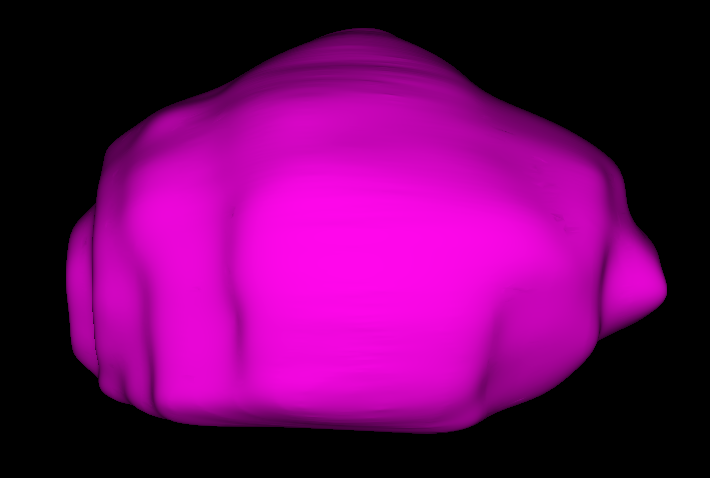
\includegraphics[width=0.3\textwidth]{zach/Cap_Modeling_Images/3D_Capsule.png} \\
Prostate Capsule \\
\begin{tabular}{ccc}
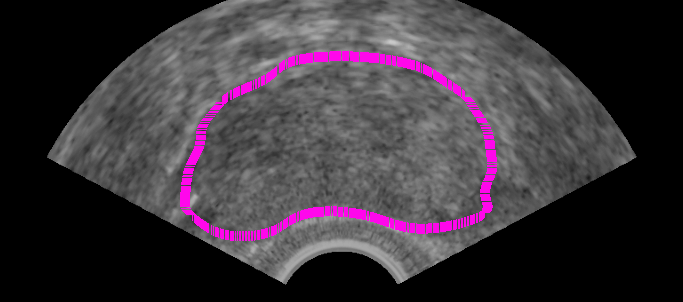
\includegraphics[width=0.3\textwidth]{zach/Cap_Modeling_Images/Axial_Cap.png} &
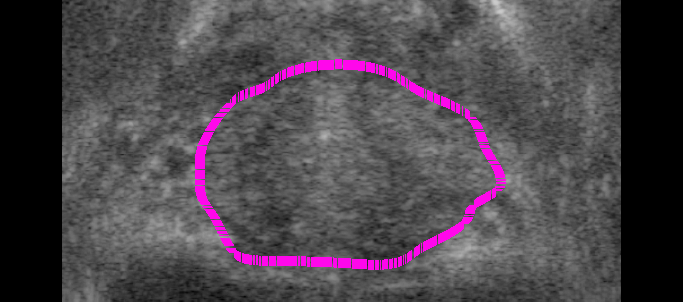
\includegraphics[width=0.3\textwidth]{zach/Cap_Modeling_Images/Coronal_Cap.png} &
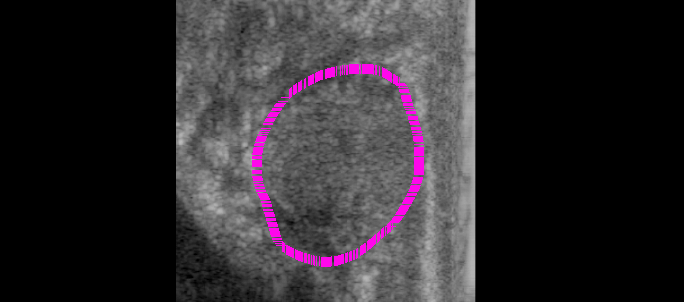
\includegraphics[width=0.3\textwidth]{zach/Cap_Modeling_Images/Sagittal_Cap.png} \\
Axial B-mode Outline & Coronal B-mode Outline & Sagital B-mode Outline \\
\end{tabular}
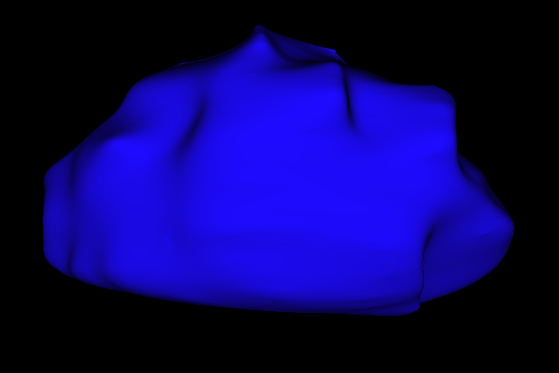
\includegraphics[width=0.3\textwidth]{zach/CG_Modeling_Images/3D_CG.png} \\
Prostate Central Gland \\
\begin{tabular}{ccc}
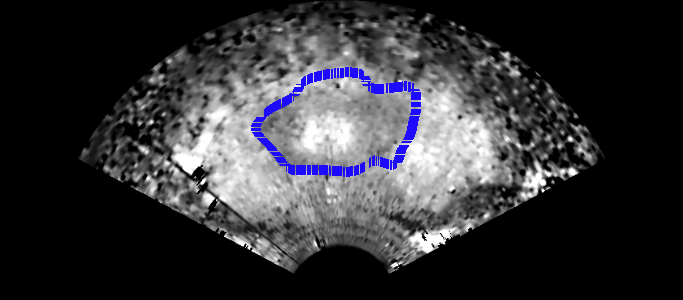
\includegraphics[width=0.3\textwidth]{zach/CG_Modeling_Images/Axial_CG.png} &
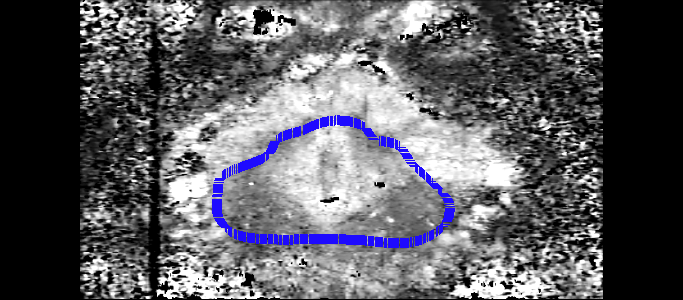
\includegraphics[width=0.3\textwidth]{zach/CG_Modeling_Images/Coronal_CG.png} &
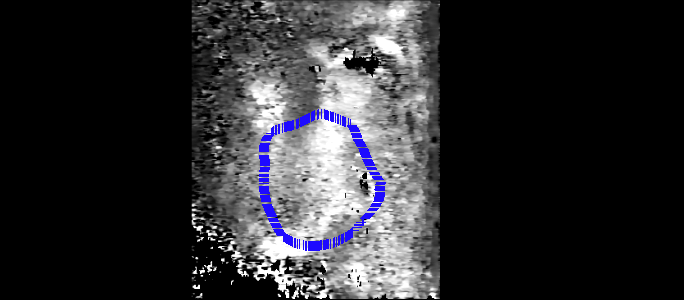
\includegraphics[width=0.3\textwidth]{zach/CG_Modeling_Images/Sagittal_CG.png} \\
Axial ARFI Outline & Coronal ARFI Outline & Sagital ARFI Outline \\
\end{tabular}
\caption{TOP ROWS: Prostate capsule 3D model (magenta) rendered from manual
    segmentation of the B-mode images, with the 3D model outlines superimposed
    on the central axial, coronal and sagital B-mode images.  The primary
    segmentation plane was sagittal; however the axial and coronal planes were
    used to guide the segmentation to insure 3D continuity of the capsule
    structure.  BOTTOM ROWS: Prostate central gland 3D model (blue) rendered
    from manual segmentation of the ARFI images, with the 3D model outlines
    superimposed on the central axial, coronal and sagital ARFI images.  The
    coronal ARFI imaging plane was the primary orientation used for image
    segmentation, but like the capsule, the orthogonal planes were used to
    insure continuity of the central gland in all three dimensions.}
\label{fig:arfi_segs} 
\end{figure}
